\section{Konteneryzacja systemu}
\label{sec:konteneryzacjaSystemu}

\par Aby przetestować działanie systemu rozproszonego, postanowiono go skonteneryzować. W tym celu skorzystano z \emph{Docekr}a\cite{DOCKER_SITE} i istniejącej w nim funkcji \emph{Compose}\cite{DOCKER_COMPOSE_DOCS}. Uprościło to proces uruchamiania, jak i umożliwiło automatyczne skonfigurowanie poszczególnych serwisów. Całość systemu została przedstawiona na diagramie \ref{fig:dockerServiceRelations}. Przedstawia on również zależności między serwisami, jakie zostały zdefiniowane w ramach plików \emph{Docker Compose}. Zależności te wyznaczają kolejność uruchomienia serwisów - wszystkie serwisy, od których zależy dany serwis, muszą zostać uprzednio uruchomione. Oznacza to, że serwisy

\begin{figure}
    \centering
    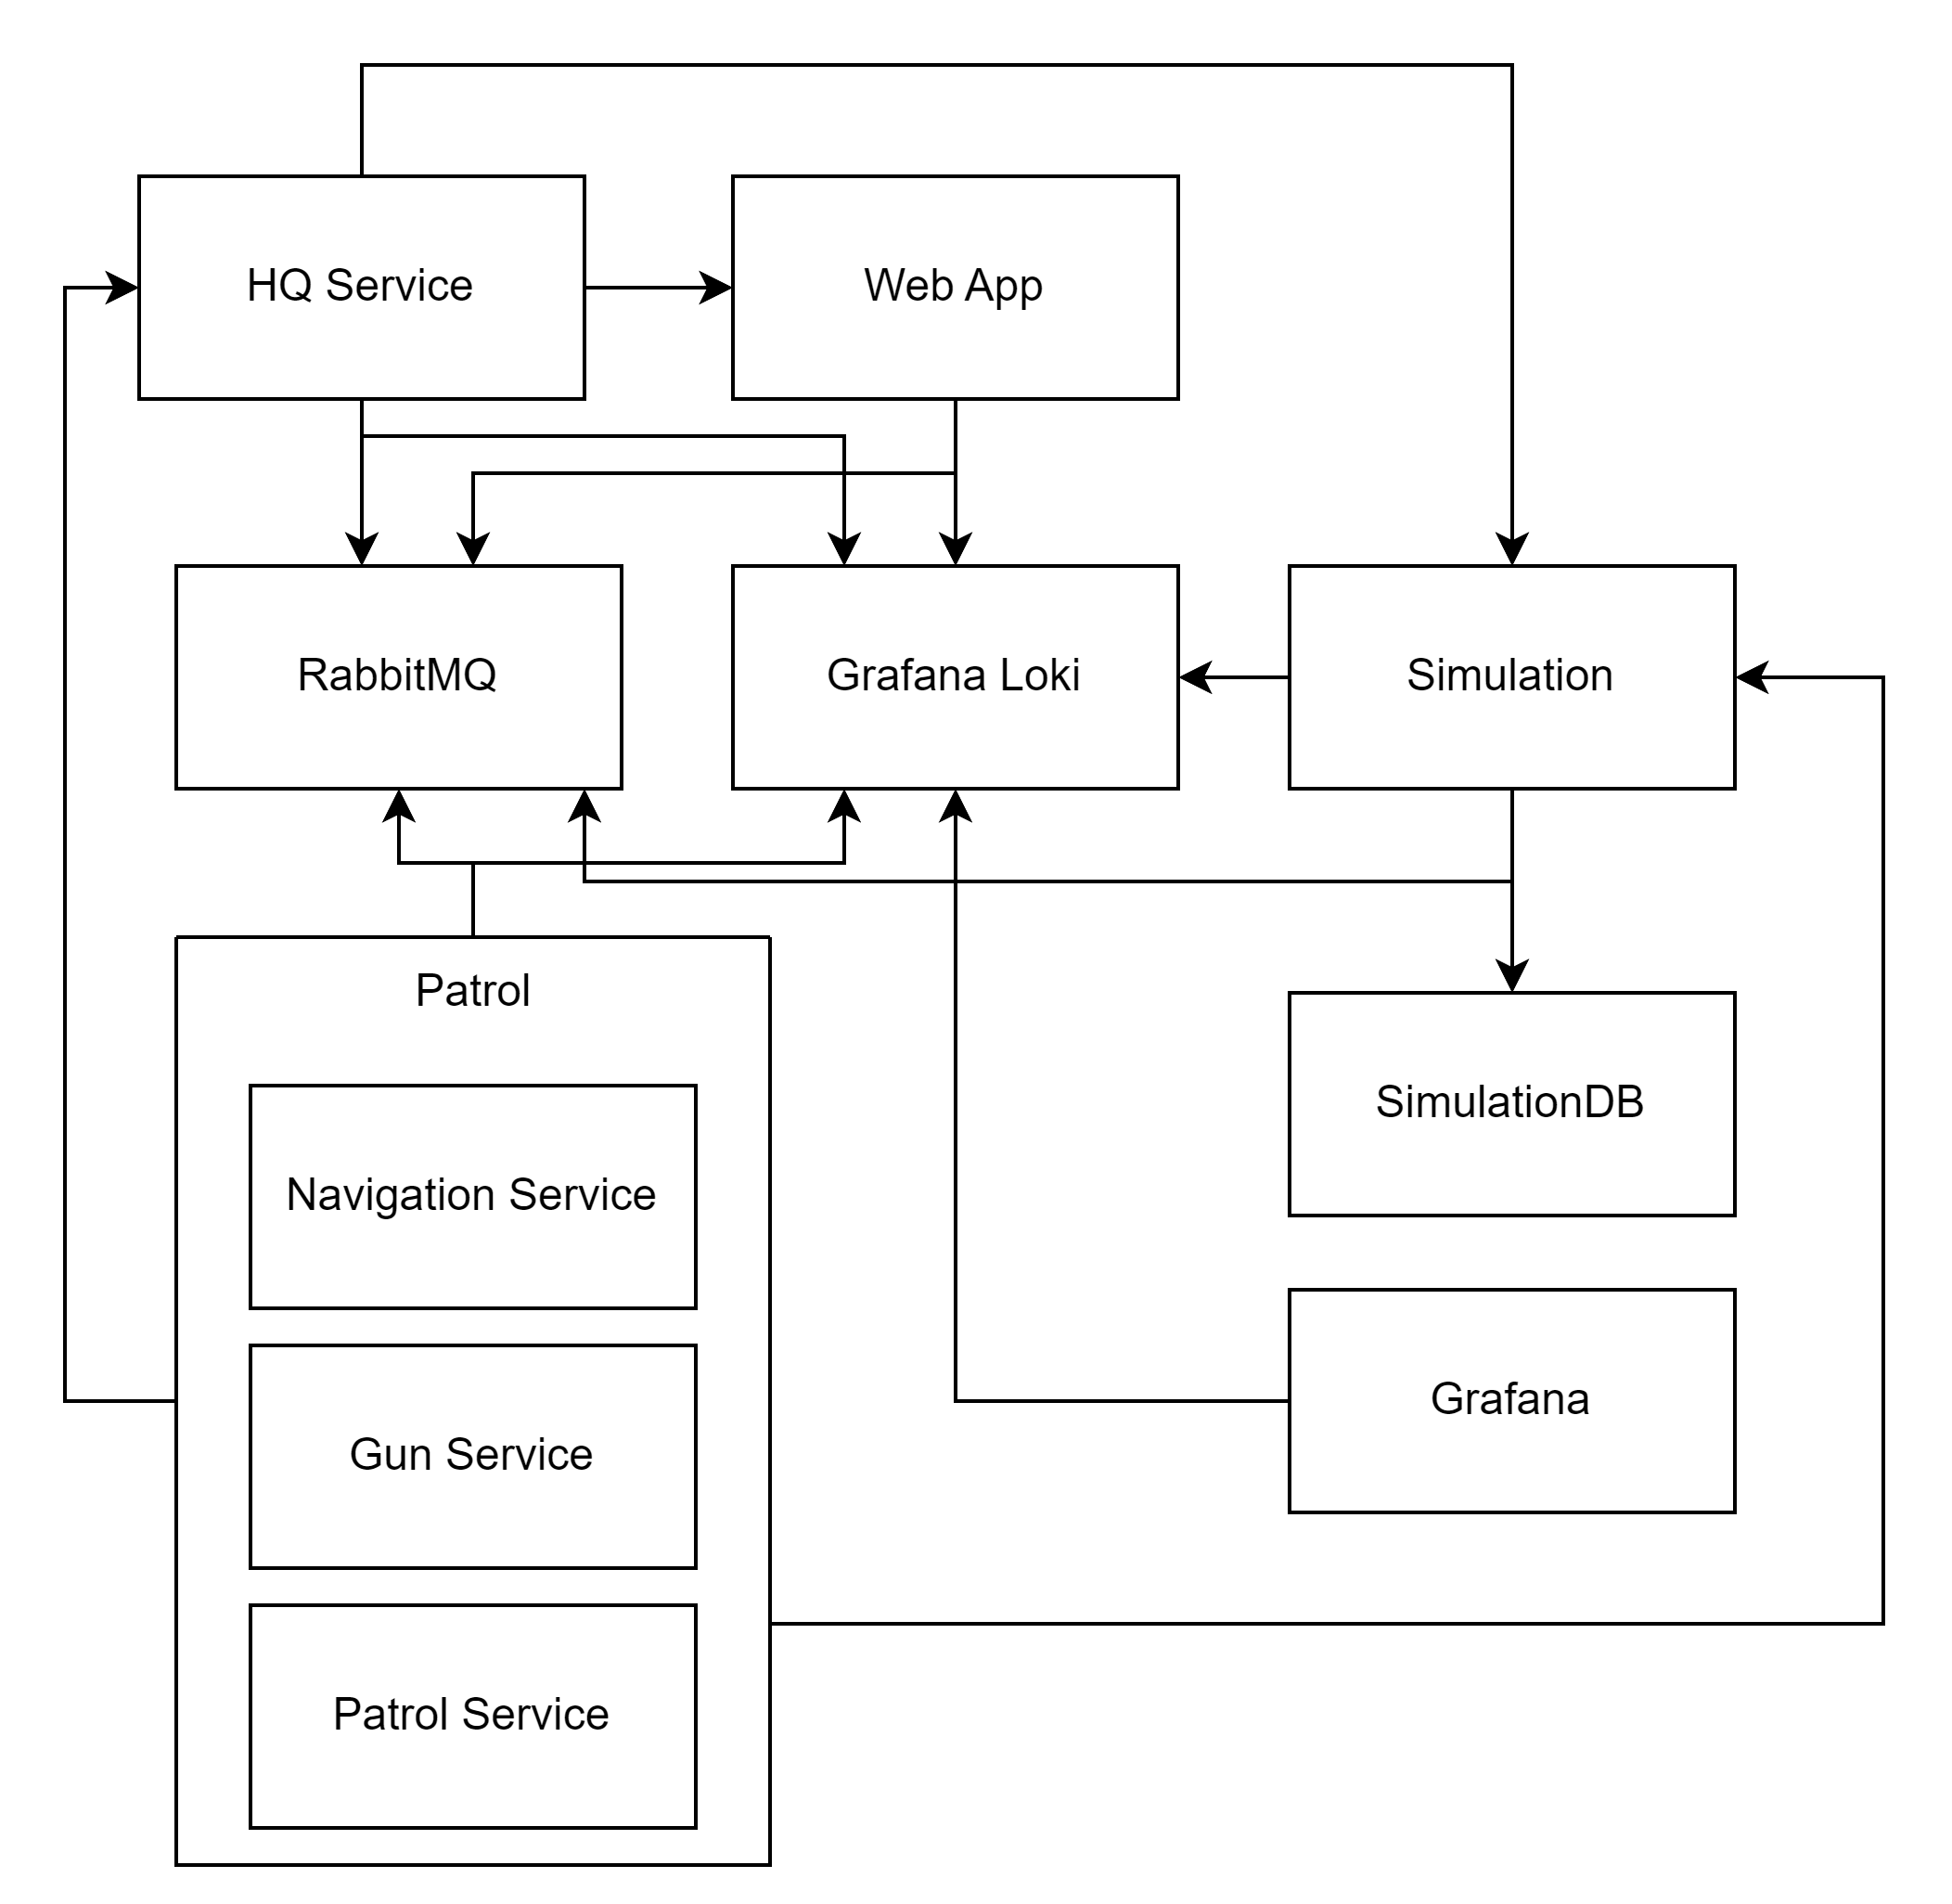
\includegraphics[width=\linewidth]{Docker - Service Dependencies}
    \caption{Diagram zależności serwisów w ramach \emph{Docker Compose}}
    \label{fig:dockerServiceRelations}
    \source{Opracowanie Własne}
\end{figure}

% TODO Dodać decision service jeżeli będzie
% TODO Dodać bazę danych, jeżeli zostanie dodana

\par Uruchamiane w ramach systemu serwisy to:
\begin{itemize}
    \item \emph{RabbitMQ},
    \item \emph{Grafana Loki},
    \item \emph{Grafana},
    \item \emph{SimulbationDB},
    \item \emph{Simulation},
    \item \emph{HQ Service},
    \item \emph{Web App},
    \item oraz serwisy patroli, składające się z \emph{Navigation Service}, \emph{Gun Service} i \emph{Patrol Service}.
\end{itemize}

\par Serwisy \emph{Grafana Loki} i \emph{Grafana} są wykorzystywane do gromadzenia i analizy logów pochodzących z systemu. Jest w nich dostępny podgląd na żywo tego co się dzieje w systemie, ale można też wykonując odpowiednie zapytania agregować i analizować uzyskane wyniki.

\par Service \emph{SimulbationDB}, to opisana w podrozdziale \ref{sec:integracjaZPostGIS} baza danych \emph{PostgreSQL}\cite{POSTGRESQL_SITE}. Wykorzystuje ona rozszerzenia \emph{PostGIS}\cite{POSTGIS_SITE} i \emph{pgRouting}\cite{PGROUTING_SITE}, aby zapewnić możliwość wyszukiwania tras na zaimportowanych mapach. Serwis ten korzysta ze specjalnie przygotowanego skrytpu \texttt{SimulationDb/start.sh}, który z wykorzystaniem \emph{osm2pgrouting}\cite{OSM2PGROUTING_GITHUB} i \emph{osm2pgsql}\cite{OSM2PGSQL_GITHUB}, importuje pliki map, wskazane w konfiguracji. Opis tej konfiguracji znajduje się w podrozdziale \ref{sec:konfiguracja}.

\par Aby zbudować i uruchomić poszczególne serwisy, powstały specjalne pliki \emph{Dockerfile} przedstawione w tabeli \ref{tab:dockerDockerFiles}. Plik \emph{patrol-combo-service-dockerfile} uruchamia w jednym kontenerze wszystkie serwisy potrzebne do działania patrolu, czyli \emph{Patrol Service}, \emph{Navigation Service} i \emph{Gun Service}. Ponieważ każdy patrol, musi posiadać unikalny identyfikator, jak i każdy z serwisów wchodzących w jego skład, musi również być identyfikowalny w sposób unikalny, to wykorzystany tutaj punkt wejścia\english{Entrypoint} nadpisuje parametry ustawione w plikach konfiguracyjnych, tymi ze zmiennych środowiskowych\english{Environment Variables}. W ten sposób można je nadpisać z poziomu, opisanego w dalszej części tego podrozdziału, pliku \emph{Docker Compose}.

\begin{table}
    \centering
    \begin{tabular}{|c|c|} 
     \hline
     Nazwa pliku & Serwis(y) \\
     \hline
     \hline
     hq-service-dockerfile & HQ Service \\ 
     \hline
     patrol-combo-service-dockerfile & Patrol Service, Navigation Service, Gun Service \\ 
     \hline
     web-app-dockerfile & Web App \\ 
     \hline
     simulation-dockerfile & Simulation \\ 
     \hline
    \end{tabular}
    \caption{Pliki \emph{Dockerfile} i serwisy, które są przez nie tworzone}
    \label{tab:dockerDockerFiles}
\end{table}

\par Dla wygody testowania, system został podzielony na warstwy w postaci 4 plików \emph{Docker Compose}. Relacje między nimi przedstawia diagram \ref{fig:dockerDockerComposeRelation}. Pierwszy z nich, czyli \texttt{infrastructure-docker-compose.yaml} służy to uruchomienia infrastruktury i serwisów pomocniczych, czyli \emph{RabbitMQ}, \emph{SimulationDB}, \emph{Grafana Loki} i \emph{Grafana}. Plik \texttt{police-services-docker-compose.yaml} rozszerza\english{Extends} rozwiązanie o główne serwisy związane z działaniem systemu, czyli \emph{Simulation}, \emph{HQ Service} i \emph{Web App}. Bazowa definicja serwisu patrolu znajduje się w \texttt{patrol-docker-compose.yaml}. Ostatni z nich, czyli \texttt{docker-compose.yaml} uruchamia całość wraz z patrolami, które są w nim zdefiniowane. Aby zmniejszyć lub zwiększyć ich ilość, należy edytować ten plik, ustawiając przy tym odpowiednie wartości w zmiennych środowiskowych:
\begin{itemize}
    \item \texttt{PoliceSupportSystem\_PatrolSettings\_\_PatrolId},
    \item \texttt{PoliceSupportSystem\_PatrolSettings\_\_PatrolAgentId},
    \item \texttt{PoliceSupportSystem\_PatrolSettings\_\_NavAgentId},
    \item \texttt{PoliceSupportSystem\_PatrolSettings\_\_GunAgentId}.
\end{itemize}
Dokładny opis działania tego mechanizmu, możemy znaleźć w podrozdziale \ref{sec:konfiguracja}.

Przykład:
\begin{Verbatim}[samepage=true]
patrol_0:
    extends:
      file: patrol-docker-compose.yaml
      service: patrol
    environment:
      - PoliceSupportSystem_PatrolSettings__PatrolId=ID
      - PoliceSupportSystem_PatrolSettings__PatrolAgentId=GUID
      - PoliceSupportSystem_PatrolSettings__NavAgentId=GUID
      - PoliceSupportSystem_PatrolSettings__GunAgentId=GUID
\end{Verbatim}

\begin{figure}
    \centering
    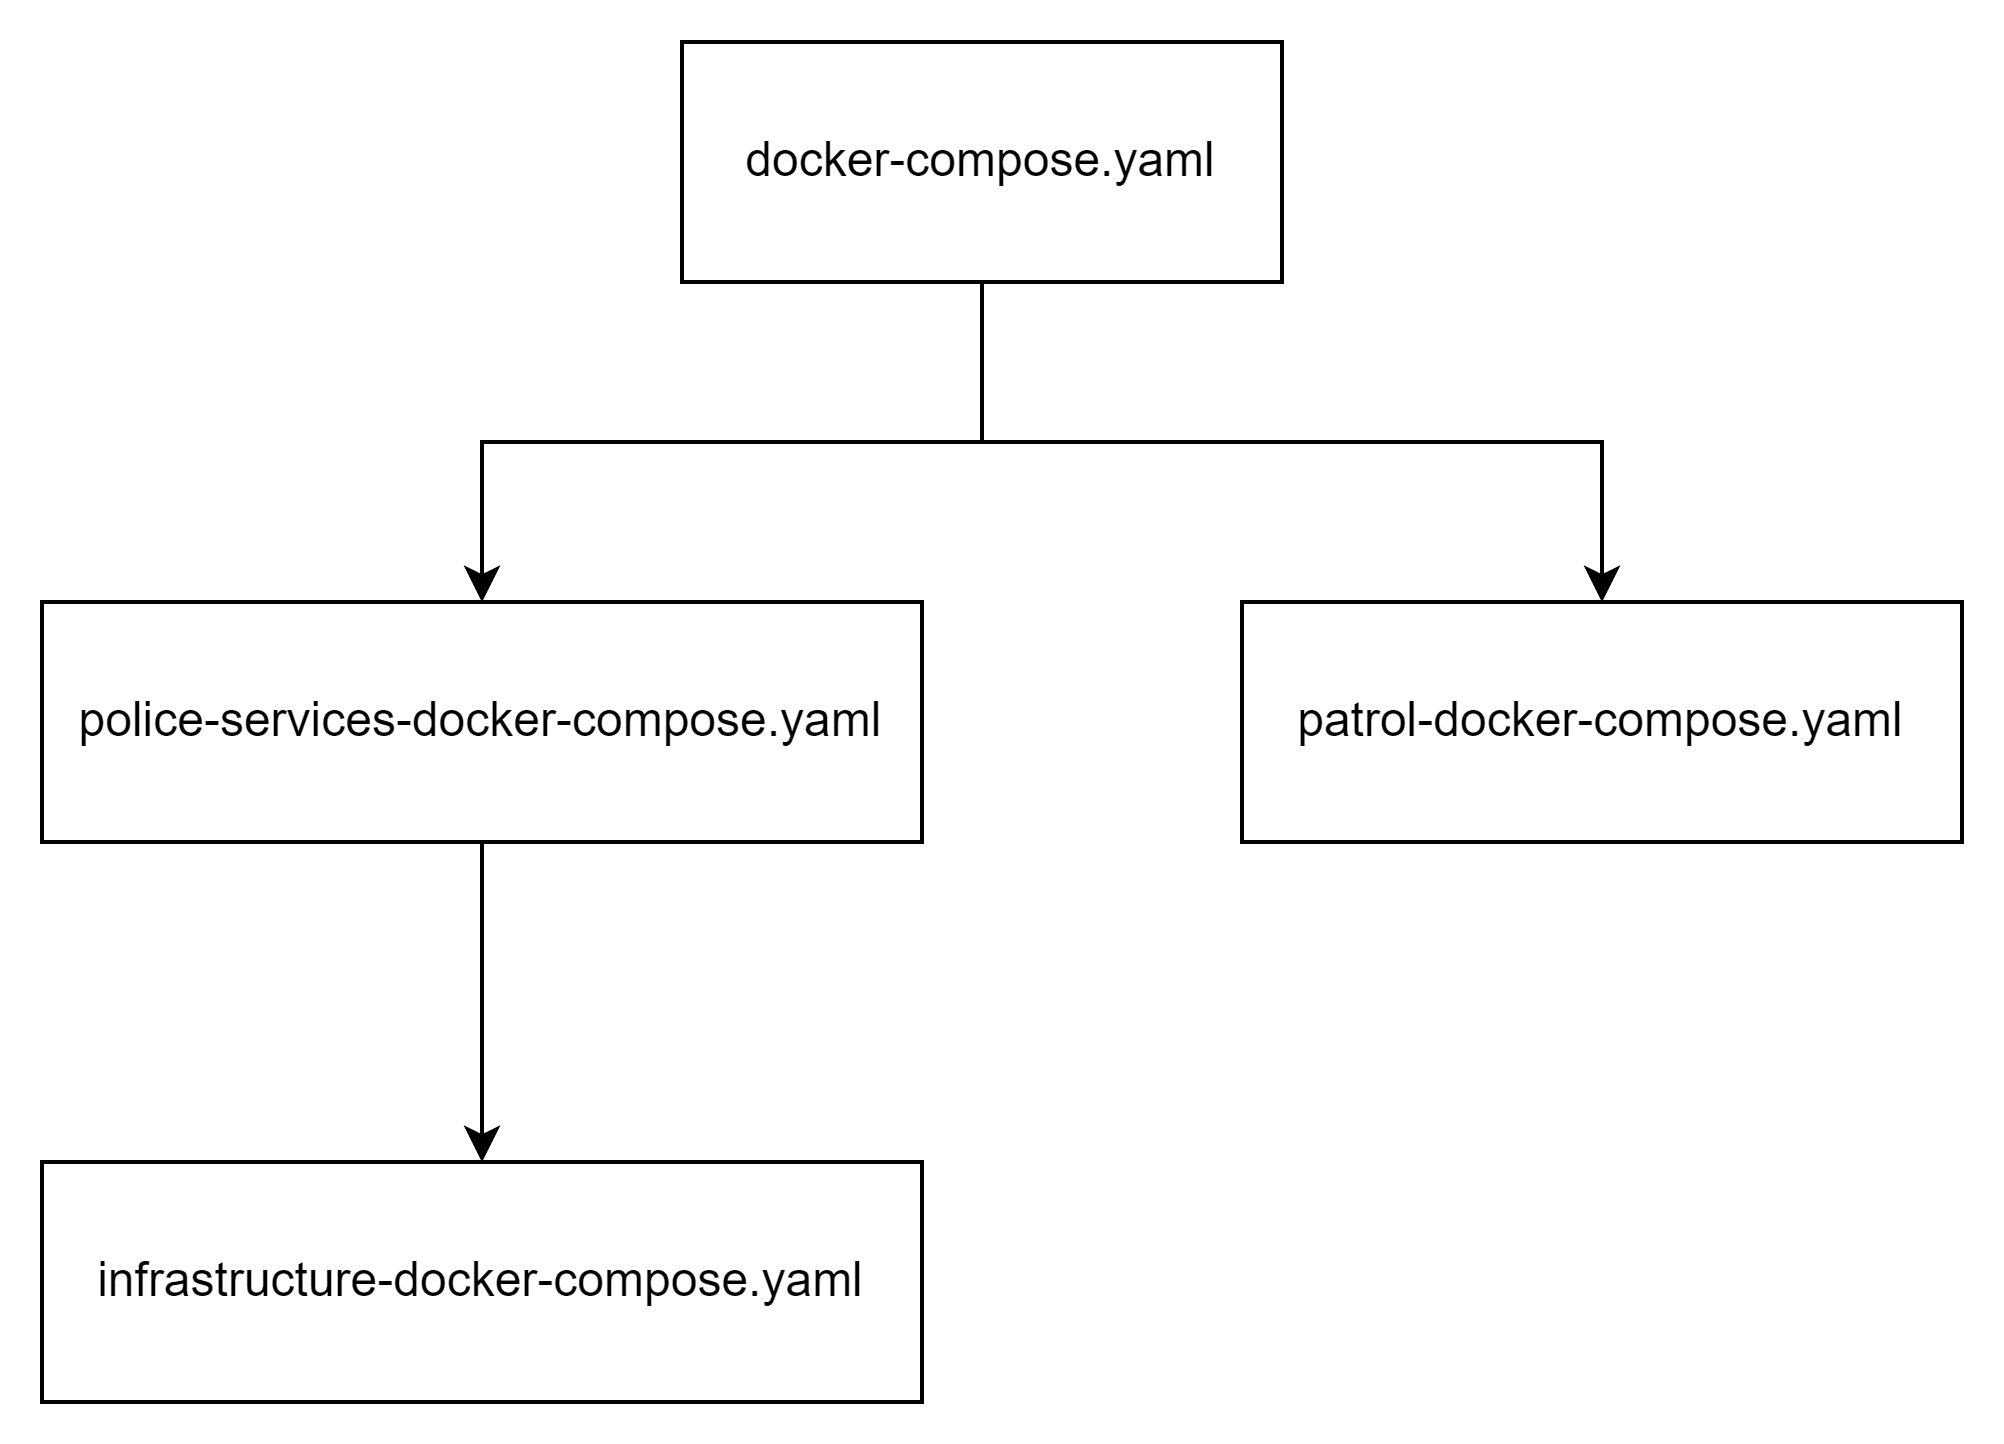
\includegraphics[width=\linewidth]{Docker - Docker Compose Relation}
    \caption{Relacje pomiędzy plikami \emph{Docker Compose}}
    \label{fig:dockerDockerComposeRelation}
    \source{Opracowanie Własne}
\end{figure}

\begin{figure}
    \centering
    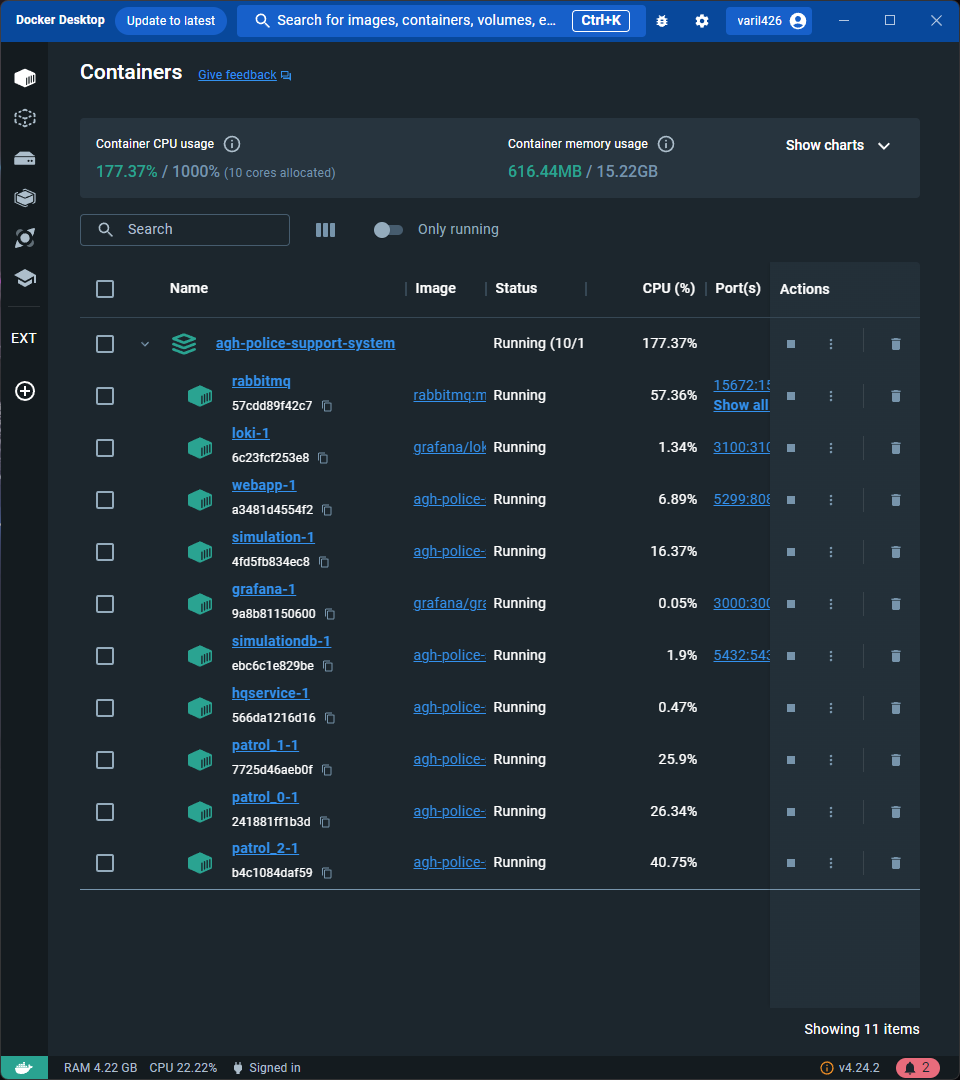
\includegraphics[width=\linewidth]{Docker - Docker Desktop}
    \caption{System z 3 patrolami uruchomiony w \emph{Docker}ze}
    \label{fig:dockerDockerDesktop}
    \source{Opracowanie Własne}
\end{figure}